%!TEX root = ../main.tex
\section{Zybo board}
The Zybo board is used in this project as it was one of the requirements for the project. 
The board features a Zynq Z-7010 chip from Xilinx, which has an integrated dual-core ARM Cortex-A9 processor and a Xilinx 7-series field programmable gate array (FPGA).
The Zybo board itself consists among other of several buttons, switches, LEDs and connections for USB, Ethernet, HDMI and several PMOD connectors.

\subsection{Functionality}
As described in the previous sections the Zybo board needs to handle a wide range of tasks.
This section will describe the different functionality that the has to be implemented.

An analysis of the complete system yielded the functionalities listed below for the Zybo board. 

\begin{itemize}
\item Digital inputs and outputs
\item Generating PWM
\item Measuring voltage output from LEM sensors
\item UART communication with external PC
\item Control algorithms for dq-control
\end{itemize}

As can be seen on the list there are multiple different tasks that needs to be handled. 
By looking at them it can be seen that optimally they should be run at different speeds.
The PWM switching frequency should be 20kHz as described in section????.
As this is quite fast it should be handled in the FPGA part of the Zynq chip. 
The rest can be handled on the ARM processor. 
In order to utilize that some tasks needs to be run at lower frequencies it was choosen to use khaOS which is a Run To Comple Scheduler (RTCS) system made by Karsten Holm Andersen. 
Using an RTCS makes it easy to schedule tasks to run at different frequencies. 
As an RTCS has no way to preempt tasks it leaves much responsibility to the programmer in order to preserve the real time performance of the system.
khaOS was chosen before other RTCS as the group had knowledge about the system from an Embedded System course.

\subsection{Architecture}
The software functionalities was grouped into tasks based on functionality and desired frequency.
A task diagram of the complete system on the Zybo can be seen in figure \ref{fig:task_diagram}.

\begin{figure}[!h]
	\centering
	\includegraphics[width=1\linewidth]{graphics/TaskDiagram}
	\caption[Task diagram.]{Task diagram of the comple system on the Zybo. Inside ARM rectangle circles are separate tasks while boxes are shared variables. In the FPGA area all the FPGA components are shown. Outside the rectangle all the signals to and from the outside world are shown.}
	\label{fig:task_diagram}
\end{figure}

As in can be seen various signals are coming from the outside world through the FPGA into the ARM processor. 
The signals from the current sensors and the the pedal will go to the ADC on the Zybo board. 
The ADC task will poll values from the ADC registers and update the $I_a$,$I_b$ and Torque reference variables.  
The UART RX and UART TX tasks are simply tasks that handle communication to a connected computer through the UART protocol.
UART TX task will read from the TX buffer and transmit the data, while the UART RX will read data coming from the connected computer and put it in the RX buffer.

\todo[inline]{add ARM label. Add RX/TX buffer. text to tx. -Mikkel}

\subsubsection{PWM generator}
The PWM generator is placed in the FPGA and is developed using Xilinx System Generator in Matlab Simulink.
The PWM generator is made to have an adjustable frequency and dutycycle.
It was choosen to make a center aligned PWM generator as this introduces less harmonic distortion than edge aligned PWM \cite{power_switching_converters}. 
Furthermore center aligned PWM also produces a symmetrical PWM signal, with a defined midpoint in the PWM-wave where the current can be sampled correctly.
The high limit for the counter can to be calculated for a given frequency, $f$, by the following:
$$Limit_H = Limit_L + \frac{f_{Zybo}}{f\cdot 2}$$
The PWM counter system can be seen in figure \ref{fig:pwm_counter}.
The counter block will count up or down depending on the input. 
The output from the counter value will go into to two compare blocks along with the high and low limits.
The compare blocks will produce a high signal when the counter value is equal to the high and low limit respectively.
These signals are then fed to a an m-code blocks which contains a simple state machine which determines if the counter should count up or down.
\begin{figure}[!h]
	\centering
	\includegraphics[width=0.7\linewidth]{graphics/counter}
	\caption[Block diagram of counter in PWM generator.]{Simulink block diagram of the counter in the PWM generator.}
	\label{fig:pwm_counter}
\end{figure}
The counter out signal can be seen in figure \ref{fig:pwm_graph}.
The counter signal is then fed into a PWM mechanism shown in figure \ref{fig:pwm}. 
The dutycycle is given to the PWM generator in the datatype u32 and therefore the dutycycle is given in range of 0 to 1000.
The switching limit will be calculeted from the following:
$$limit_{switching} = (1 - \frac{duty_{thousand}}{1000}) \cdot range_{counter}$$
A register will then make sure that the switching limit is only passed on when the counter is at its lowest.
The compare block will make the PWM signal by comparing the switcing limit to the counter value.
The counter signal and output of the PWM generator can be seen in figure \ref{fig:pwm_graph}.
As the PWM generator should be able to do three independent PWM signal there are three of the systems shown in figure \ref{fig:pwm}, one for each phase.

\begin{figure}[!h]
	\centering
	\includegraphics[width=0.8\linewidth]{graphics/pwm_system}
	\caption[Block diagram of PWM generator.]{Simulink block diagram of the PWM mechanism in the PWM generator.}
	\label{fig:pwm}
\end{figure}


\begin{figure}[!h]
	\begin{center}
		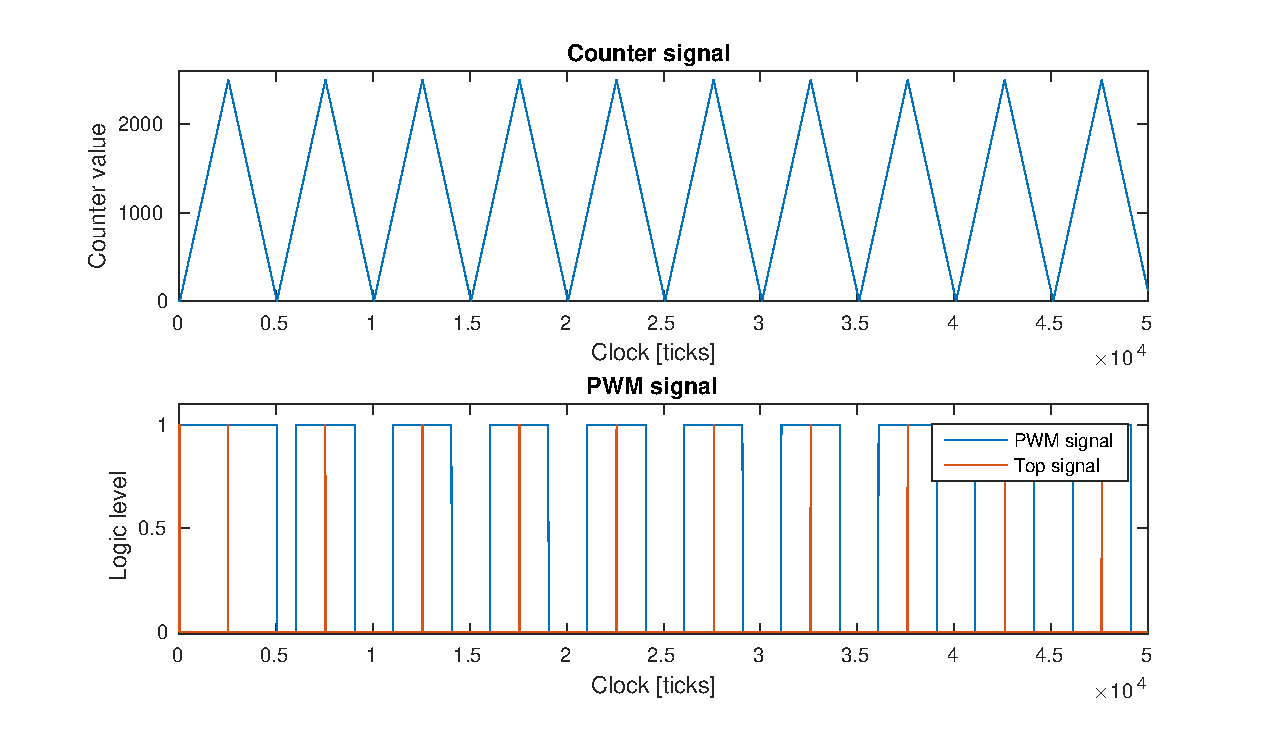
\includegraphics[width=\linewidth]{graphics/pwm_plot}
		\label{fig:pwm_graph}
		\caption{Counter and PWM signal.}
	\end{center}
\end{figure}

\subsubsection{Interface task}
The interface task is the task that has to read external signals, output digital signals and control the other tasks.
The UART tasks will be controlled through two buffers, while the controller and PWM task will have to read the enable variable updated by the interface task.
The basic funcionality of the interface task can be seen in the flowchart of figure \ref{fig:interface}.
\begin{figure}[!h]
	\centering
	\includegraphics[width=0.7\linewidth]{graphics/interface_task}
	\caption[Block diagram of PWM generator.]{Simulink block diagram of the counter in the PWM generator.}
	\label{fig:interface}
\end{figure}
\todo[inline]{Can there be less whitespace in the figure? -MIkkel}
\todo[inline]{Is the inrush relay explained somewhere?? -MIkkel}



\subsubsection{Controller task}
The controller tasks basic functionality can be seen in figuer \ref{fig:controller_task}.
It reads from the variables $I_a$ and $I_b$ and calculates $I_c$. 
$I_a$, $I_b$, $I_c$ and $\theta$ are then used to perform a Clarke Park transformation. 
$I_d$ and $I_q$ are then controlled with two seperate PI controllers. 
$I_d$ is controlled with reference $0$ and $I_q$ is controlled with the pedal as reference.

\begin{figure}[!h]
	\centering
		\includegraphics[width=0.7\linewidth]{graphics/controller_task}
	\caption[Block diagram of controller task.]{Block diagram showing the functionality of the controller task.}
	\label{fig:controller_task}
\end{figure}



\subsubsection{PWM task}
The PWM tasks basic functionality can be seen in the block diagram of figure \ref{fig:pwm_task}.
The PWM task is a seperate task from the controller task as it might be preferrable to have the two tasks run at different frequencies.
It is responsible for performing inverse Clarke Park transformation using $V_{sd}$, $V_{sq}$ and $\theta$. 
Afterwards the calculated dutycycles will be written to the PWM generator in the FPGA if the enable signal is high.

\begin{figure}[!h]
	\centering
		\includegraphics[width=0.7\linewidth]{graphics/pwm_task}
	\caption[Block diagram of PWM task.]{Block diagram showing the functionality of the PWM task.}
	\label{fig:pwm_task}
\end{figure}

\todo[inline]{Smaller figure and less whitespace and change the order of vsd and vsq? -MIkkel}
\todo[inline]{Where should we talk about the concept of dq and the meaning of it? -MIkkel}
\todo[inline]{Third harmonic injection and why? -MIkkel}

\subsubsection{ADC}
Something here...

\subsection{TEST or whatever}



%\subsection{Analysis}
%\subsection{Conclusion}